\chapter{Experiments}\label{sec:experiments}

Here all the described algorithms are going to be applied to different datasets. As described, the Multi Relocalizer consists of two parts \textit{Place Finder} and \textit{Real Pose Finder}, both parts will be analysed independently and finally together. Then, the global method using \textit{ferns} will be analysed.\\

Measures are in SVO metric which is initialized when the program starts, it should be approximated to meters. Errors should be considered as relative to other solutions and not as absolute.\\

\section{Desktop dataset}

The first used dataset has been captured on a desktop. The first part of the dataset will be used for training the relocalizer while the second part will be used for testing. From both parts the pose is known. It will be used, not only to visualize the error as ground truth, but also in the \textit{naive Place Finder} described later.\\

In figure~\ref{fig:desktop_2_train_test} both the training and testing data can be seen together, where every set contains 10 images. It should be noted that the data does not coincide, only using closest frame will not yell good results, and so the \textit{Real Pose Finder} step is very important. In~\ref{fig:desktop_2_example_image} there is an example of the images in the dataset.\\

\begin{figure}[htpb]
  \begin{subfigure}[b]{6cm}
          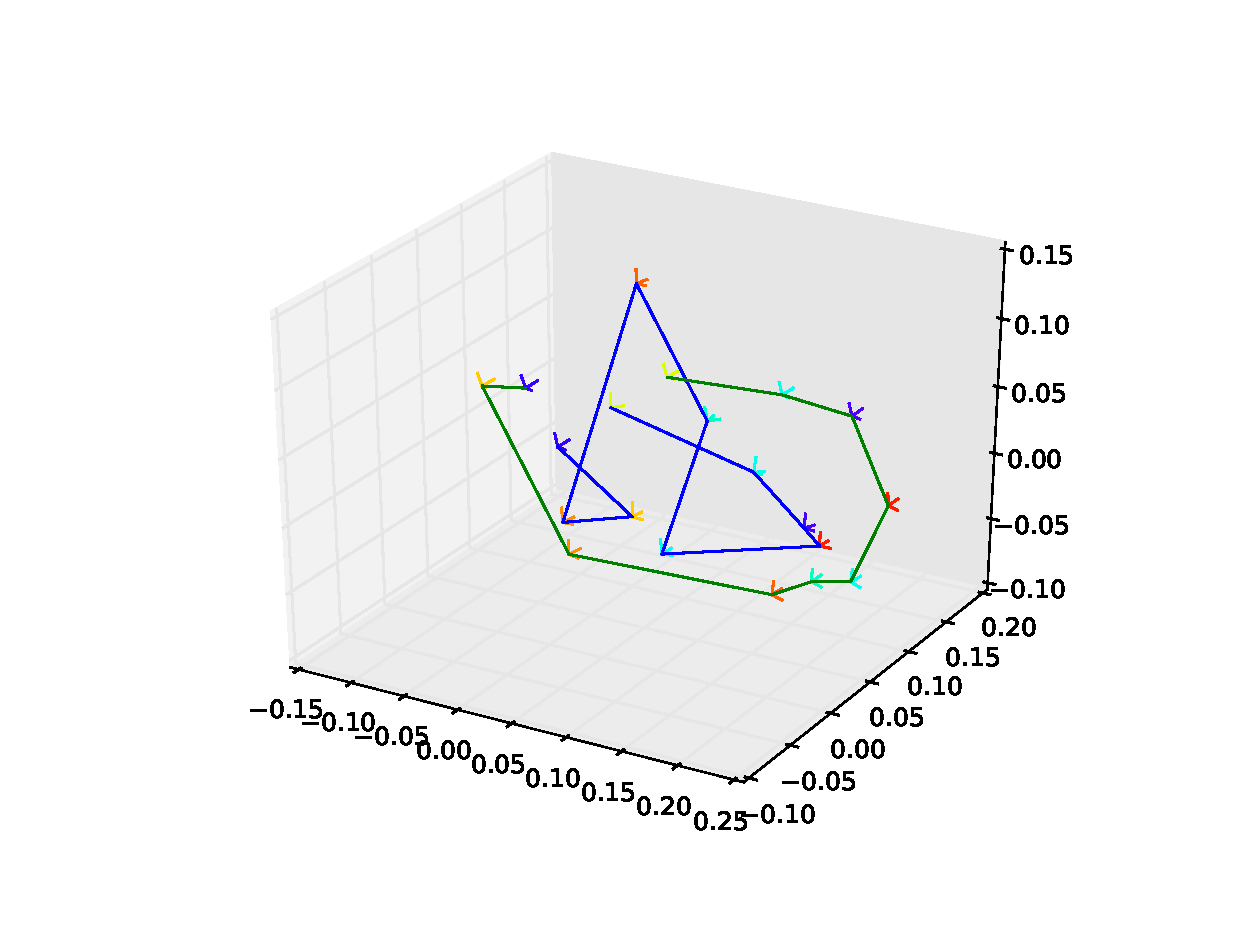
\includegraphics[width=\linewidth]{img/desktop_2_train_test.eps}
          \caption{In green, the path used for training. In blue, the path used for testing}                
          \label{fig:desktop_2_train_test}
  \end{subfigure}   
  \qquad
  \begin{subfigure}[b]{5cm}
         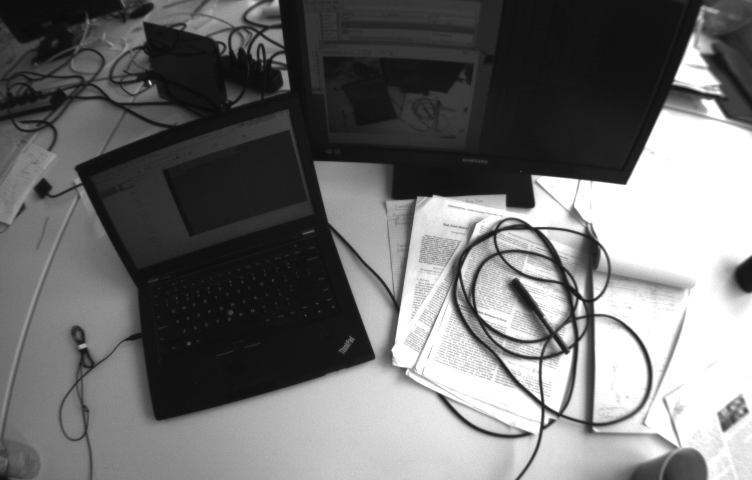
\includegraphics[width=\linewidth]{img/image00654.png}
         \caption{Example of an image from the dataset}                
         \label{fig:desktop_2_example_image}
  \end{subfigure}
  \caption{}
\end{figure}

\subsection{Multi Relocalizer}
\label{sub:multi_relocalizer}

\subsubsection{Naive \textit{Place Finder}}
\label{ssub:naive_and_emptry}

To analyse the performance of the different \textit{Real Pose Finder} methods a \textit{naive} implementation of a \textit{Place Finder} is used, it uses the ground truth information to find the real closest frame, being it an ideal \textit{Place Recognition} method. In~\ref{fig:desktop_2_naive_empty_path_1} there is the result using this method, it can be seen that even being ideal it is not so good. Next, different \textit{Real Pose Finder} will be used to correct this situation.\\

\begin{figure}[htpb]
  \begin{subfigure}[b]{6cm}
          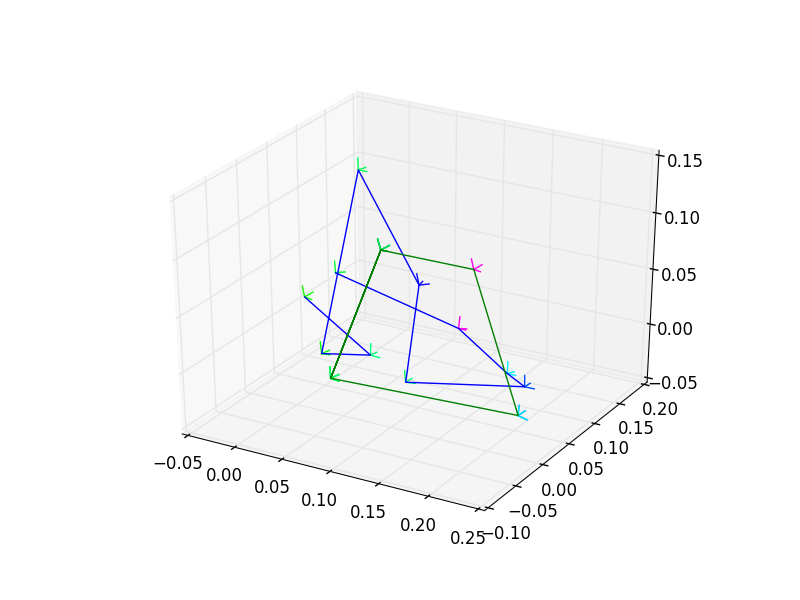
\includegraphics[width=\linewidth]{img/desktop_2_naive_empty_path_1.png}
          \caption{In blue, testing ground truth. In green, found path}                
          \label{fig:desktop_2_naive_empty_path_1}
  \end{subfigure}   
  \qquad
  \begin{subfigure}[b]{6cm}
         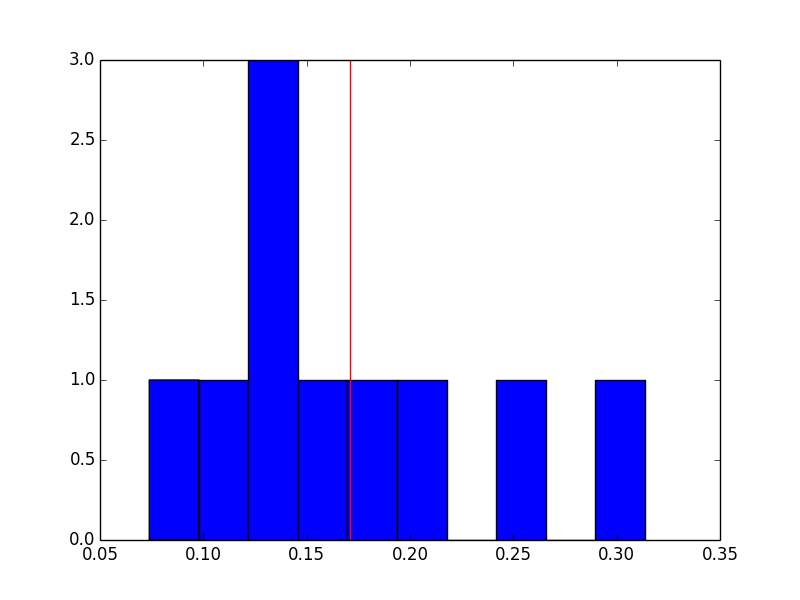
\includegraphics[width=\linewidth]{img/desktop_2_naive_empty_dist_1.png}
         \caption{Translation error histogram, mean in red}                
         \label{fig:desktop_2_naive_empty_dist_1}
  \end{subfigure}
  \caption{Results using the Naive \textit{Place Finder} an no \textit{Real Pose Finder}}
\end{figure}

To evaluate the results in a numeric way a histogram of the translation error have been plotted in~\ref{fig:desktop_2_naive_empty_dist_1}, it is going to be used as a baseline to see how posterior methods can improve it.\\

\subsubsection{Cross Covariance \textit{Place Finder}}
\label{ssub:cross_covariance_place_finder}

As said, the naive approach is the optimal \textit{Place Finder}, this implementation is not as good but would like it to be as close as possible. Looking at the error histogram~\ref{fig:desktop_2_CC_empty_dist_1} it can be seen that the mean error is higher but int general the results are similar, if the naive approach can be corrected this method should also be corrected. This error is used as a baseline to see how the results can be improved.\\

\begin{figure}[htpb]
  \begin{subfigure}[b]{6cm}
          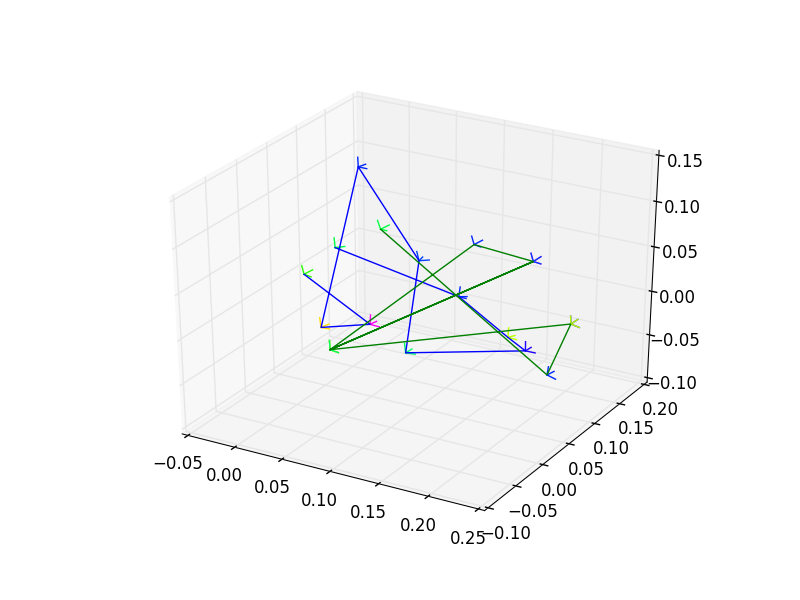
\includegraphics[width=\linewidth]{img/desktop_2_CC_empty_path_1.png}
          \caption{In blue, testing ground truth. In green, found path}                
          \label{fig:desktop_2_CC_empty_path_1}
  \end{subfigure}   
  \qquad
  \begin{subfigure}[b]{6cm}
         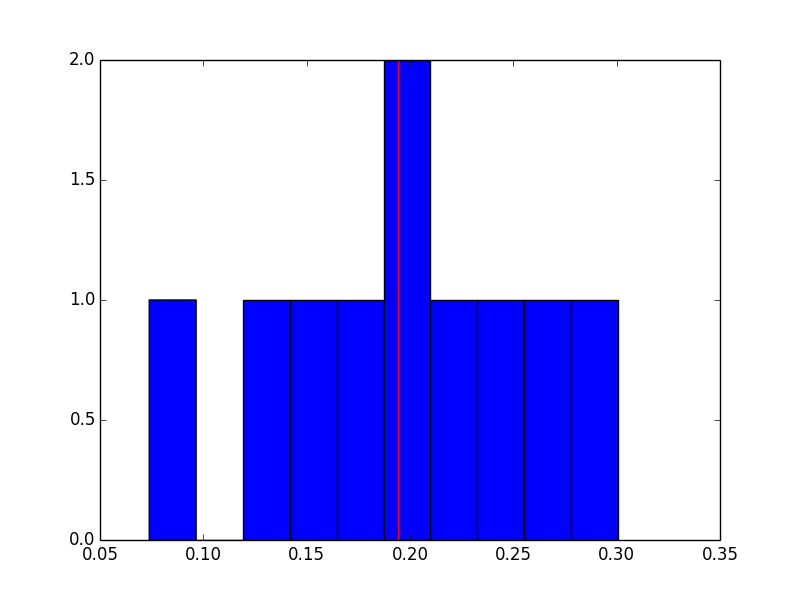
\includegraphics[width=\linewidth]{img/desktop_2_CC_empty_dist_1.png}
         \caption{Translation error histogram, mean in red} 
         \label{fig:desktop_2_CC_empty_dist_1}
  \end{subfigure}
  \caption{Results using Cross Covariance \textit{Place Finder} and no \textit{Real Pose Finder}}
\end{figure}

\subsubsection{Extended Second-other Minimization \textit{Real Pose Finder}}
\label{ssub:extended_second_orther_minimization_textit_real_pose_finder}

This is the method used in PTAM. First, the method has been applied together with the naive \textit{Place Finder} and the with CC. Although the found paths in \ref{fig:desktop_2_naive_esm_path_1} and~\ref{fig:desktop_2_CC_esm_path_1} are not easily evaluated visually, looking at~\ref{fig:desktop_2_naive_esm_dist_1} and~\ref{fig:desktop_2_CC_esm_dist_1} and comparing them to their corresponding baseline previously mentioned, it can be seen that in both cases the results improve.\\

The algorithm performs better with the mentioned ideal \textit{Place Finder}, so alternative and more accurate implementations should be considered to improve the results of this \textit{Real Pose Finder}.\\


\begin{figure}[htpb]
  \begin{subfigure}[b]{6cm}
          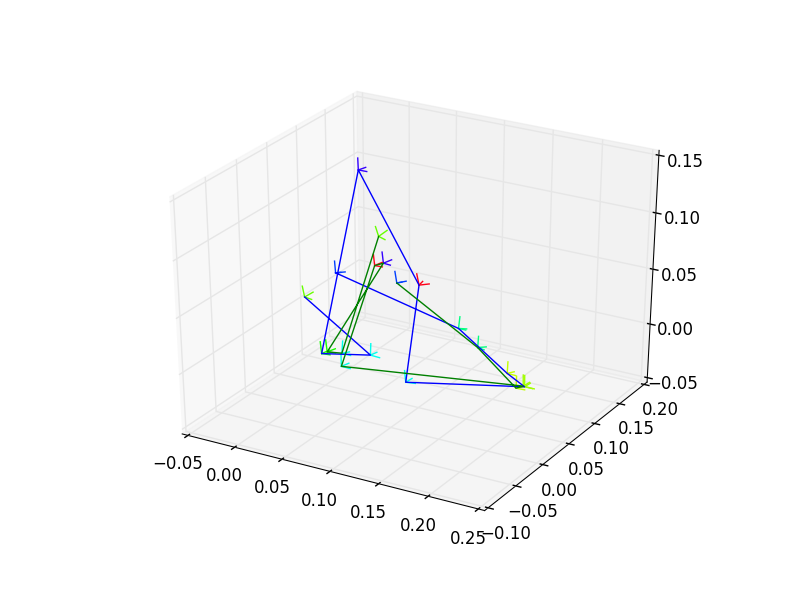
\includegraphics[width=\linewidth]{img/desktop_2_naive_esm_path_1.png}
          \caption{In blue, testing ground truth. In green, found path}                
          \label{fig:desktop_2_naive_esm_path_1}
  \end{subfigure}   
  \qquad
  \begin{subfigure}[b]{6cm}
          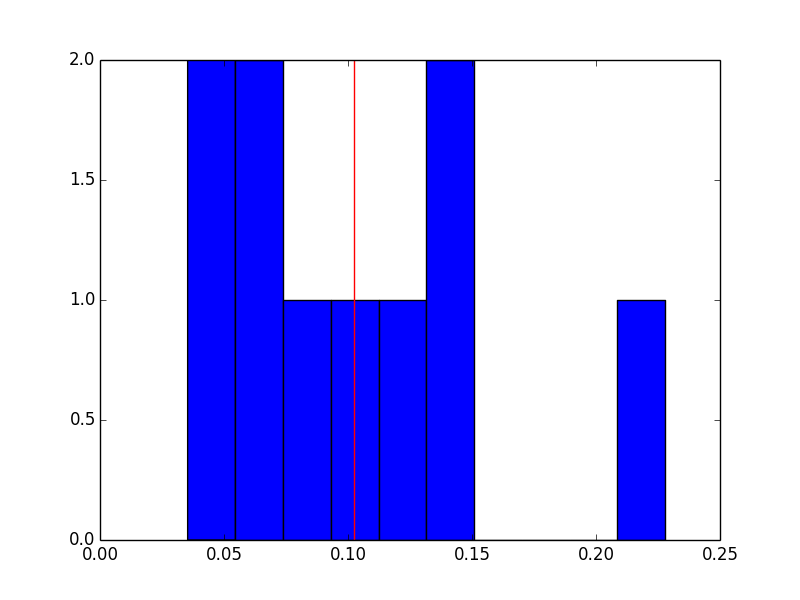
\includegraphics[width=\linewidth]{img/desktop_2_naive_esm_dist_1.png}
          \caption{Translation error histogram, mean in red} 
          \label{fig:desktop_2_naive_esm_dist_1}
  \end{subfigure}
  \caption{Results using Naive \textit{Place Finder} and ESM  \textit{Real Pose Finder}}
\end{figure}


\begin{figure}[htpb]
  \begin{subfigure}[b]{6cm}
          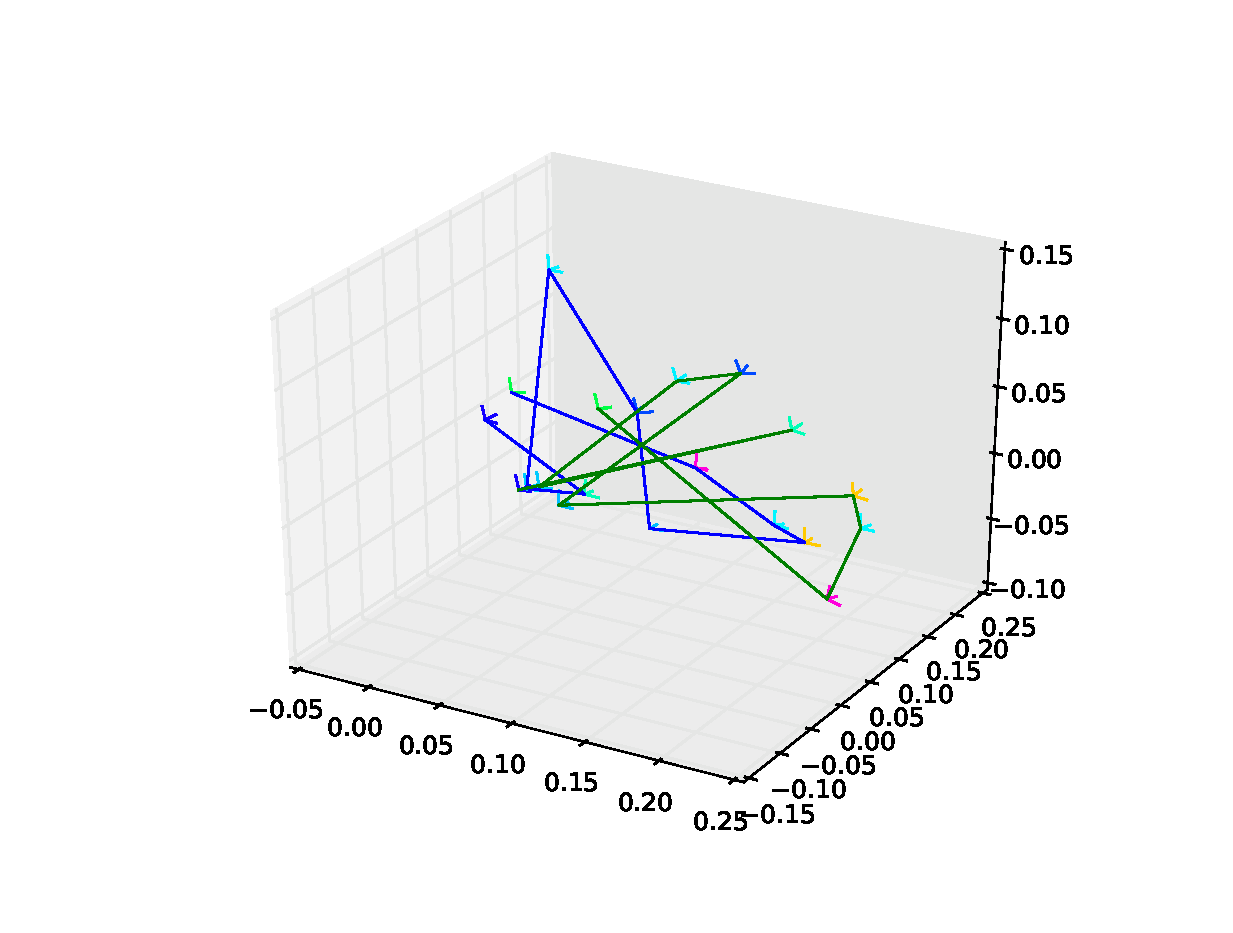
\includegraphics[width=\linewidth]{img/desktop_2_CC_esm_path_1.eps}
          \caption{In blue, testing ground truth. In green, found path}                
          \label{fig:desktop_2_CC_esm_path_1}
  \end{subfigure}   
  \qquad
  \begin{subfigure}[b]{6cm}
          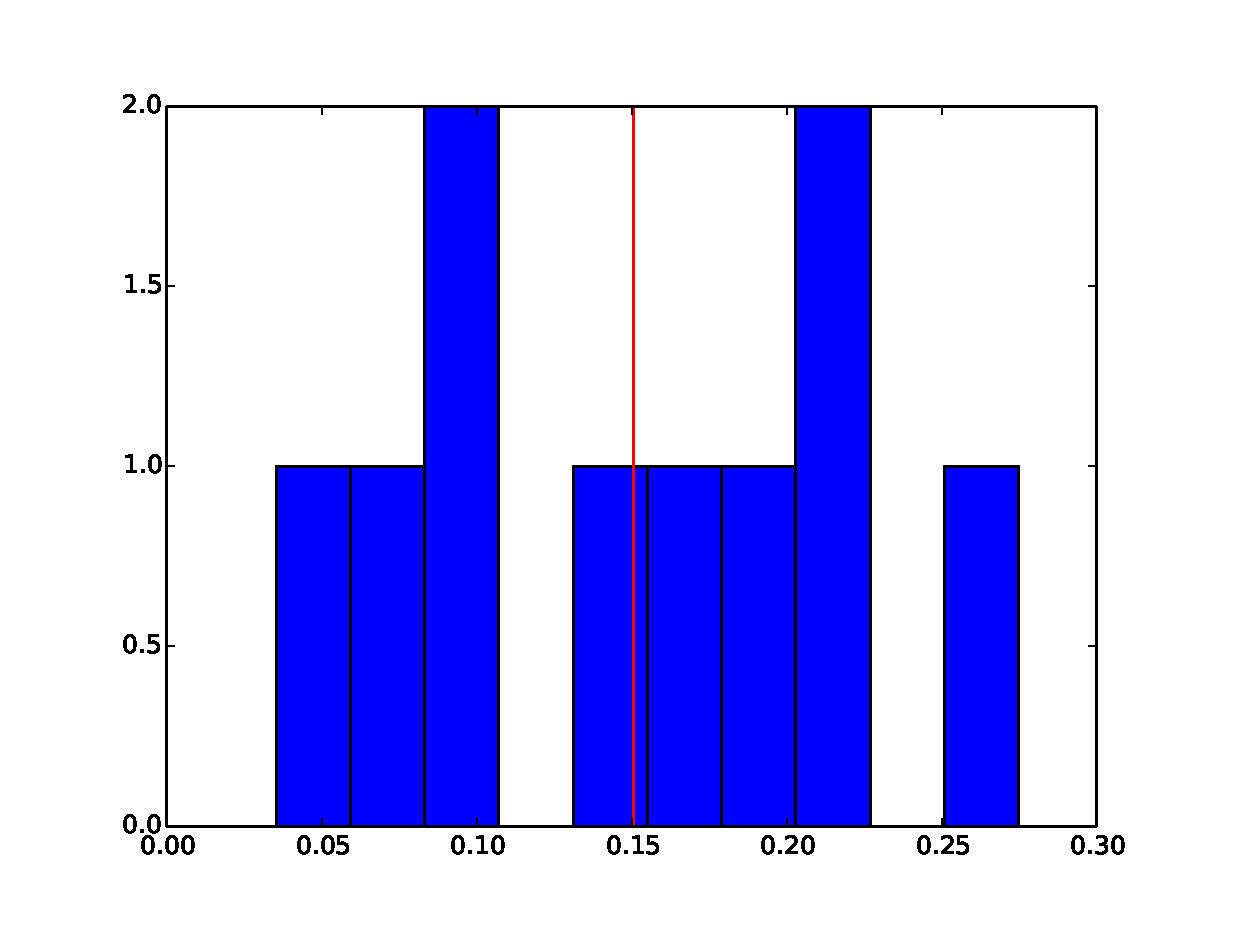
\includegraphics[width=\linewidth]{img/desktop_2_CC_esm_dist_1.eps}
          \caption{Translation error histogram, mean in red} 
          \label{fig:desktop_2_CC_esm_dist_1}
  \end{subfigure}
  \caption{Results using CC \textit{Place Finder} and ESM  \textit{Real Pose Finder}}
\end{figure}


\subsubsection{Three-point \textit{Real Pose Finder}}
\label{ssub:three_point_real_pose_finder}

As an alternative to the method proposed by PTAM we applied the feature extraction and matching framework to find the transformation between two frames knowing the world frame location of the features. Tracking the world location of features is something that is no available on all VO implementations and it can be very useful to solve the described problem.\\

\begin{figure}[htpb]
  \begin{subfigure}[b]{6cm}
          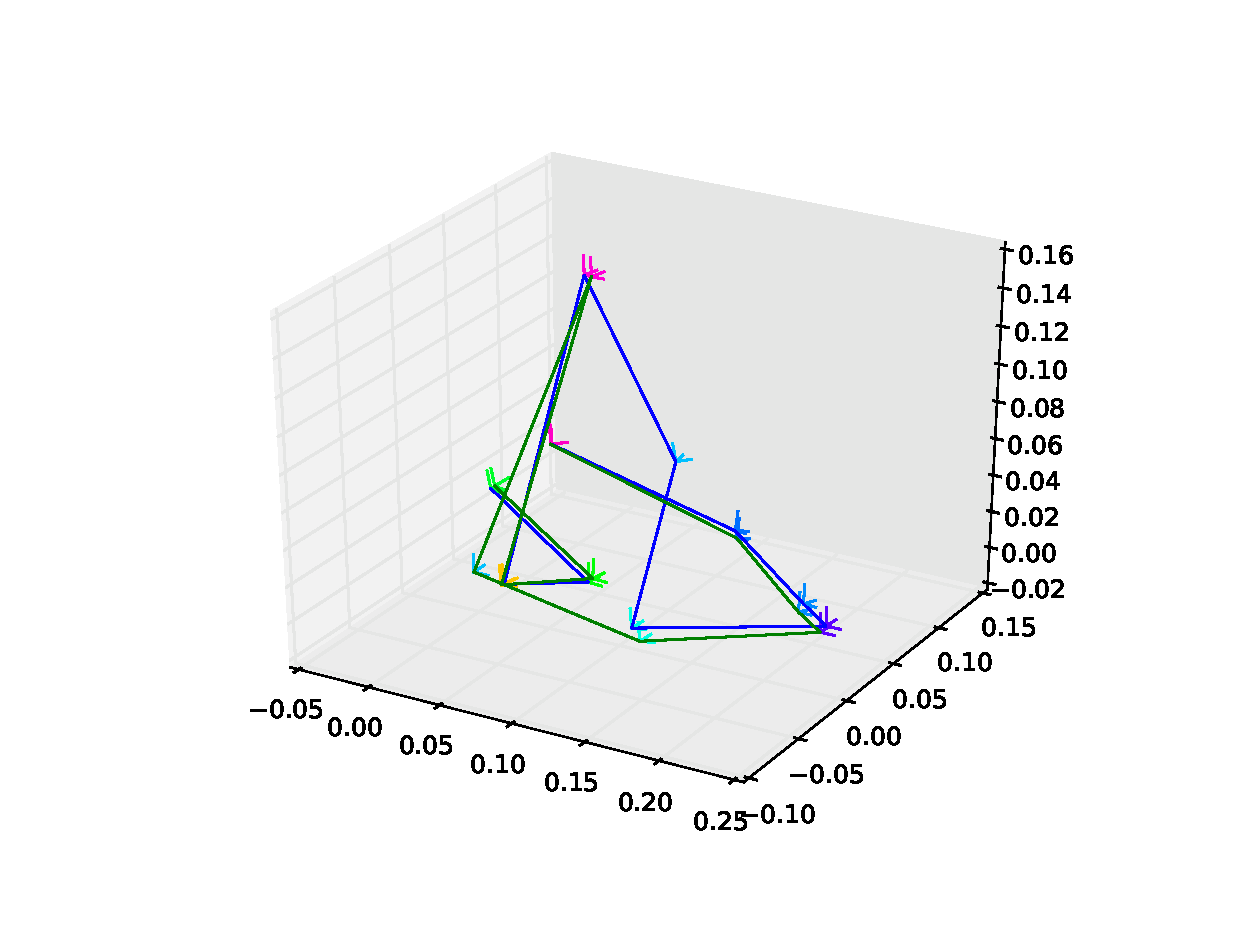
\includegraphics[width=\linewidth]{img/desktop_2_naive_3pt_path_1.eps}
          \caption{In blue, testing ground truth. In green, found path}                
          \label{fig:desktop_2_naive_3pt_path_1}
  \end{subfigure}   
  \qquad
  \begin{subfigure}[b]{6cm}
          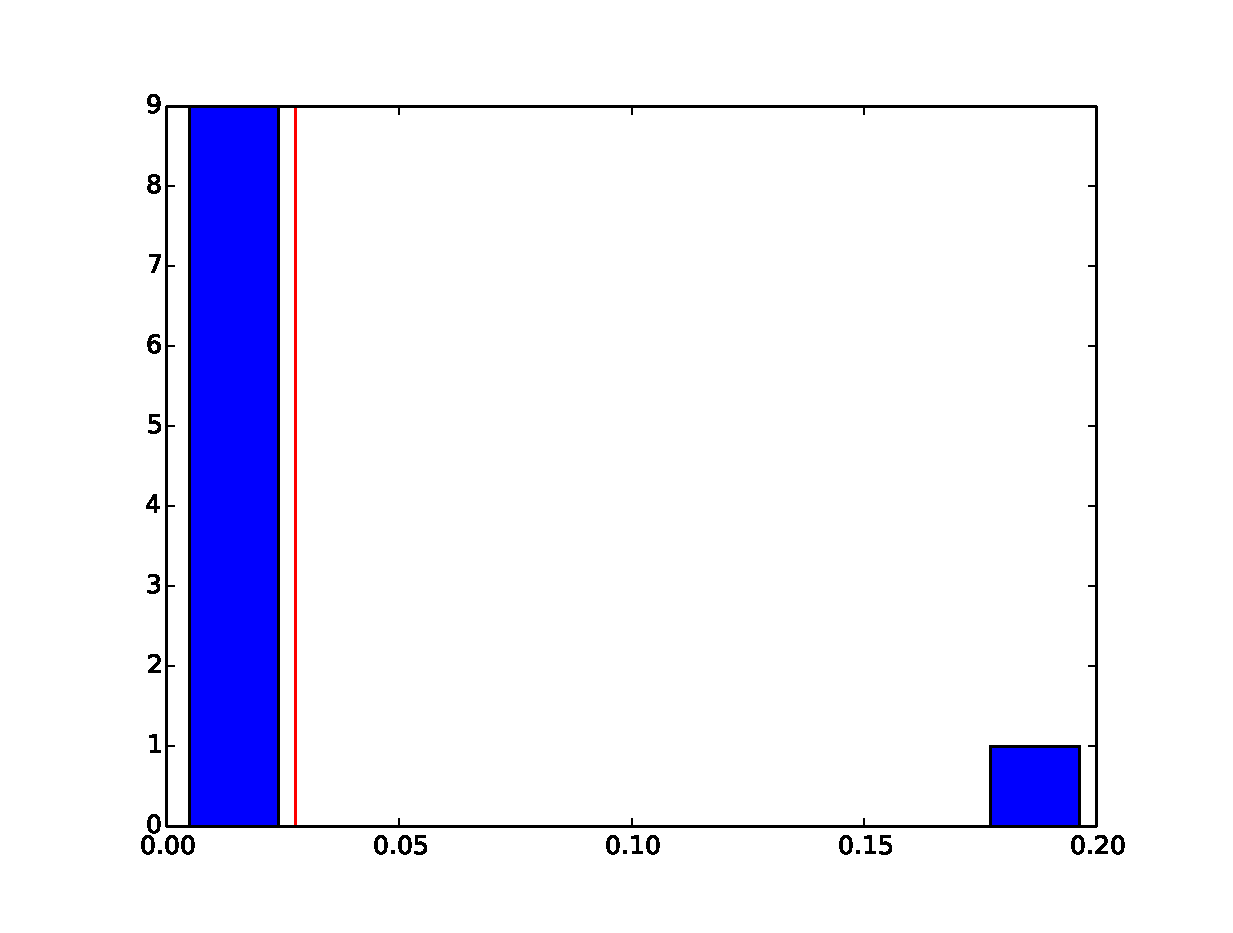
\includegraphics[width=\linewidth]{img/desktop_2_naive_3pt_dist_1.eps}
          \caption{Translation error histogram, mean in red} 
          \label{fig:desktop_2_naive_3pt_dist_1}
  \end{subfigure}
  \caption{Results using Naive \textit{Place Finder} and 3pt  \textit{Real Pose Finder}}
\end{figure}

In the case of the naive approach, in~\ref{fig:desktop_2_naive_3pt_dist_1}, the results are very good. Using this method the pose of the frames is recovered, in most cases, perfectly yelling a very low mean error. There is one frame which was not correctly relocalized, in that case not enough match were found between the pair of images. As seen in~\ref{fig:not_enough_matches} only two matches where found and , even correct, these are not enough to run the three-point algorithm. A large change in viewpoint can affect severely the descriptors performance been this the cause of the missing matches.\\

\begin{figure}[htpb]
  \centering
  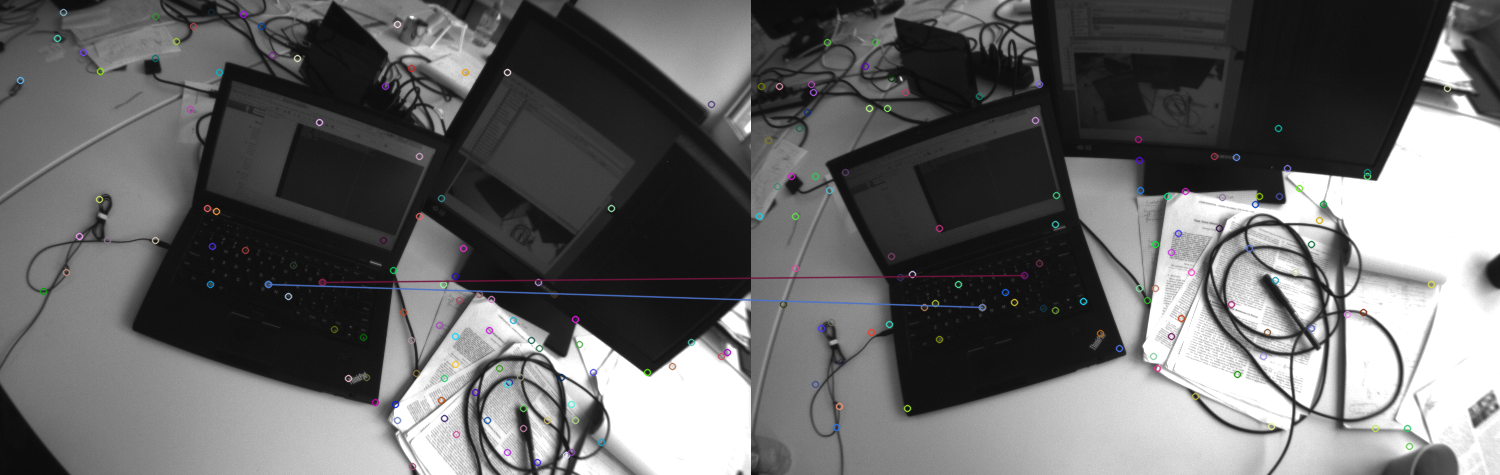
\includegraphics[width=11cm]{img/not_enough_matches.png}
  \caption{Found matches. Not enough to run the three-point algorithm}
  \label{fig:not_enough_matches}
\end{figure}

On the other case~\ref{fig:desktop_2_CC_3pt_dist_1}, using CC, the results are also good. Here, there is one of the frames whose pose is not correctly recovered. In this case, as seen in~\ref{fig:wrong_inlier}, there are enough matches but during RANSAC one match from three is taken in as valid leading to a wrong solution.\\

\begin{figure}[htpb]
  \begin{subfigure}[b]{6cm}
          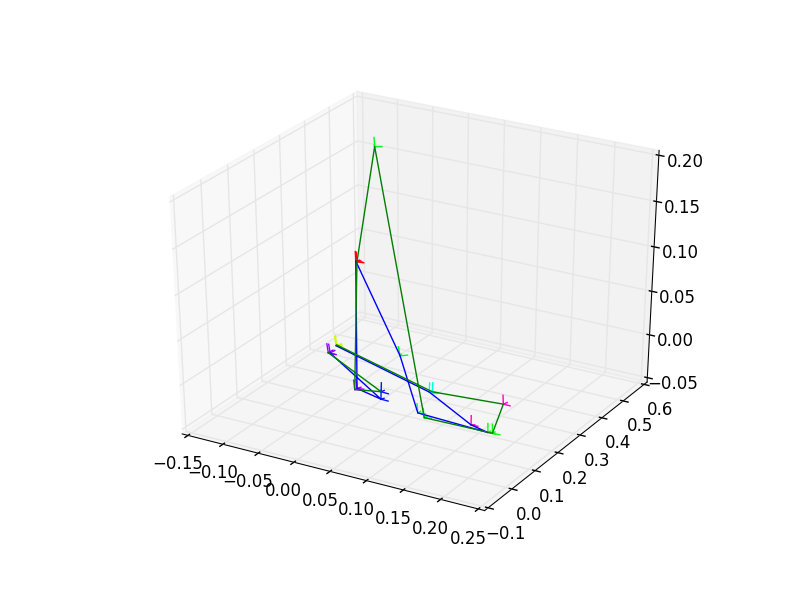
\includegraphics[width=\linewidth]{img/desktop_2_CC_3pt_path_1.png}
          \caption{In blue, testing ground truth. In green, found path}                
          \label{fig:desktop_2_CC_3pt_path_1}
  \end{subfigure}   
  \qquad
  \begin{subfigure}[b]{6cm}
          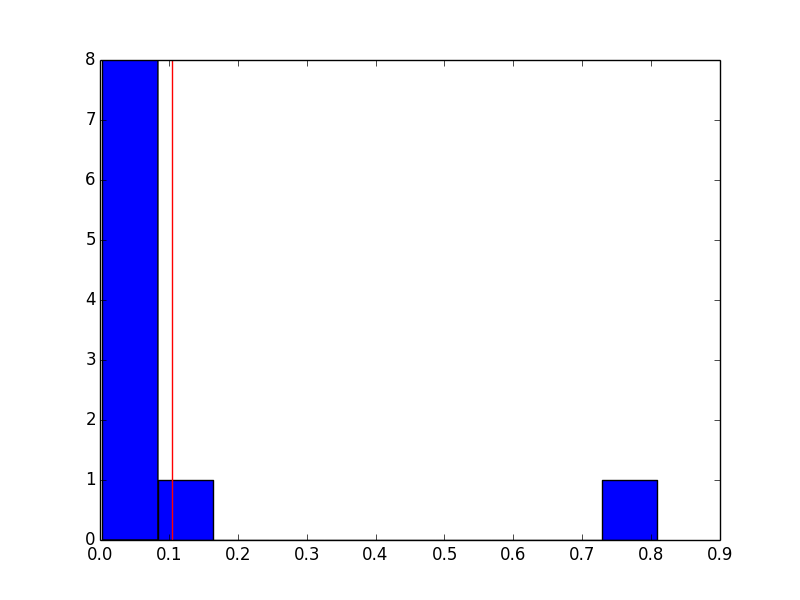
\includegraphics[width=\linewidth]{img/desktop_2_CC_3pt_dist_1.png}
          \caption{Translation error histogram, mean in red} 
          \label{fig:desktop_2_CC_3pt_dist_1}
  \end{subfigure}
  \caption{Results using CC \textit{Place Finder} and 3pt  \textit{Real Pose Finder}}
\end{figure}

\begin{figure}[htpb]
  \centering
  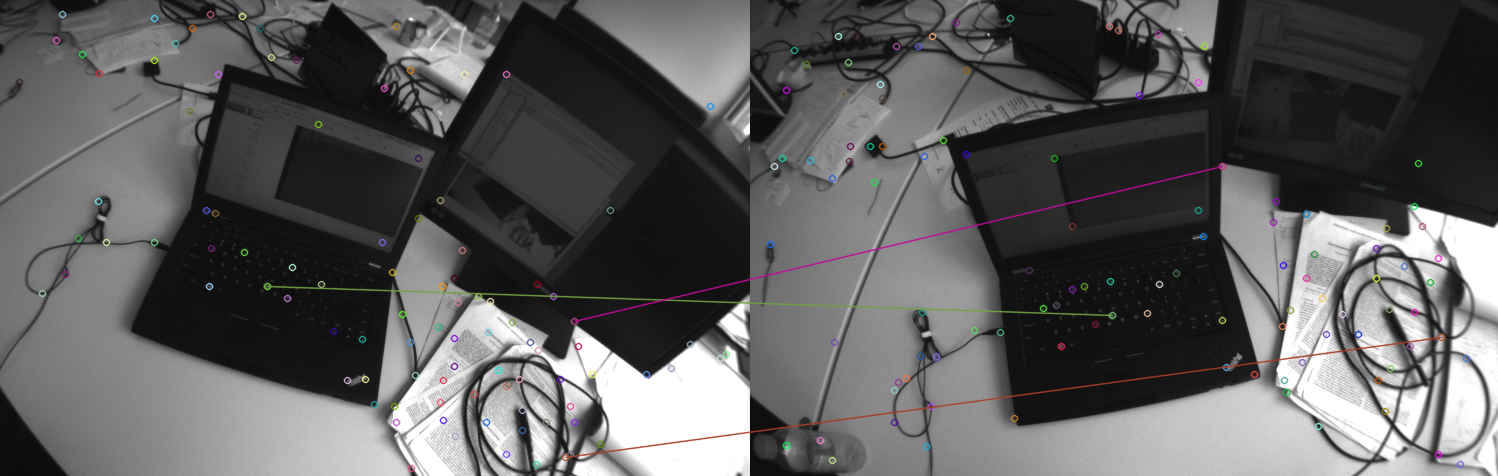
\includegraphics[width=11cm]{img/wrong_inlier.png}
  \caption{}
  \label{fig:wrong_inlier}
\end{figure}
